\newpage
\section{Durchführung}
\label{sec:Durchführung}
\subsection{Justierung}
\begin{figure}
  \centering
  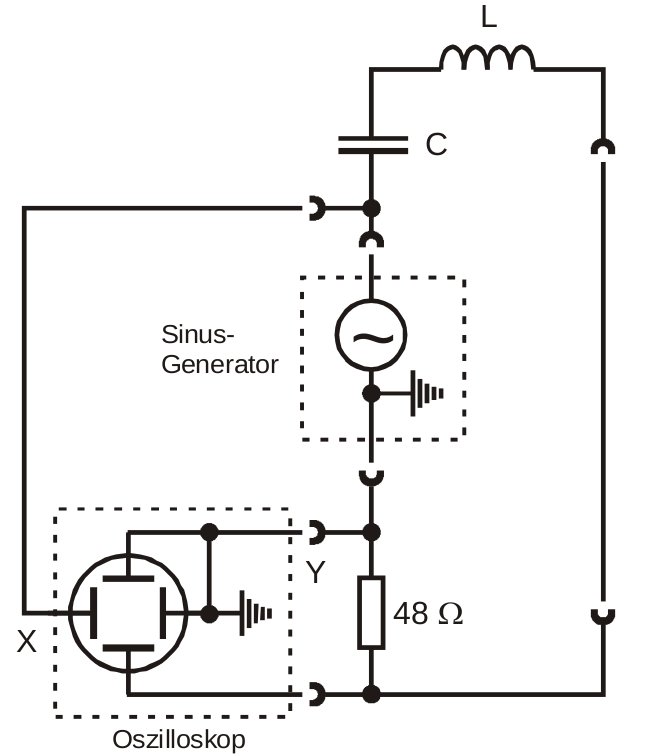
\includegraphics[height= 7cm]{./logos/Abb5.png}
  \caption{Schaltung zur Bestimmung der Resonanzfrequenz eines Schwingkreises}
  \label{fig:Abb5}
\end{figure}
\FloatBarrier
Zu aller erst wird die Schlatung aus Abbildung \ref{fig:Abb5} und messen die Resonanzfrequenz, die ungefähr beim Strommaximum liegt. Die Feinabstimmung
erfolgt dann durch Lissajous-Figuren, diese verschwinden im Falle der Resonanz. Zunächst wird  noch eine Schaltung wie in Abb. \ref{fig:Abb5} aufgebaut, jedoch mit dem
abstimmbaren Schwingkreis. In diesem wird die Resonanzfrequenz auf den gemessenen Wert angeglichen.
\newpage
\subsection{Messprogramm}
\subsubsection{Schwingungs-und Schwebungsfrequenz}
\begin{figure}
  \centering
  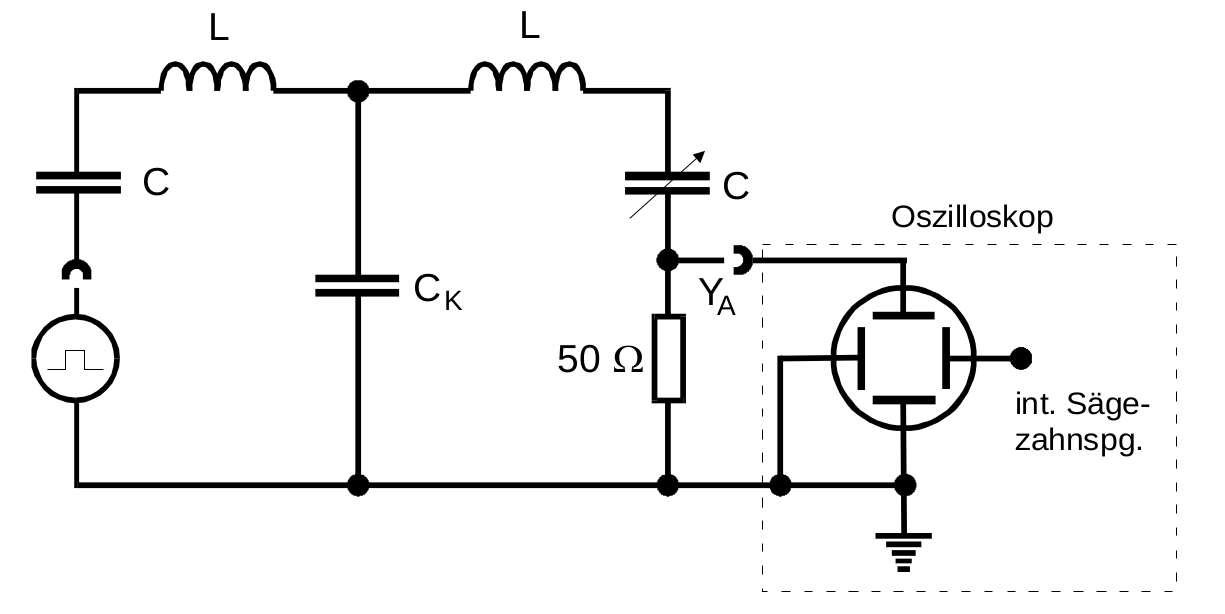
\includegraphics[width=\textwidth]{./logos/Abb6.png}
  \caption{Schlatung zur Untersuchung von zwei gekoppelten Schwingkreisen}
  \label{fig:Abb6}
\end{figure}
\FloatBarrier
Nun wird die Schaltung aus Abbildung \ref{fig:Abb6} aufgebaut. Der linke Schwingkreis wird mit einem Nadelimpuls oder einer Rechteckspannung angeregt.
Auf dem Oszilloskop lassen sich dann das Verhältnis von Schwingungs-und Schwebungsfrequenz ablesen. Hierzu werden die Schwingungsmaxima innerhalb der Schwebungsperiode gezählt.
Das Verhältnis der Frequenzen wir für jede Variation von $C_K$ mit $ 2 \leq C_K \leq 12 nF $ gemessen.
\subsubsection{Fundermentalschwingungen in Abhänigkeit von $C_K$  bestimmt mit Lissajous-Figuren}
  In diesem Teil des Versuches wird der Nadelimpusl bzw. die Rechteckspannung aus Abb. \ref{fig:Abb6} durch ein Sinussignal ersetzt. Nun wird wieder $C_K$ variiert und für
  jeden Wert $ \nu_+$ und $\nu_-$ bestimmt. Die Lissajous-Figuren helfen hier die Frequenzen zu finden bei denen die Phase Null oder $ \pi $ ist.
\subsubsection{Fundermentalschwingungen in Abhänigkeit von $C_K$  bestimmt mit Sweep-Methode}
  Jetzt wird die Sinusspannung mit einem Sweep versehen. Dieser lässt die Sinusspannung in einem einstellbarem Zeitintervall von einer bestimmten Frequenz auf eine andere ansteigen.
  Auf dem Osilloskop kann man dann den Anfang und das Ende des Sweeps beobachten bei korrekter Einstellung kann man dort die Resonanzpeaks beobachten. Dabei misst man
  die Zeitintervalle vom Anfang des Sweeps zu einem der Resonanzpeaks. Auch bei diesem Teil des Versuches werden alle Werte abhängig vom Koppelkondensators $ C_K$ bestimmt.
